\documentclass[11pt,a4paper]{article}
\usepackage[margin=22mm,top=23mm,bottom=23mm,headheight=14pt,footskip=12mm]{geometry}
\usepackage{fontspec}
\setmainfont{Noto Sans}
\setsansfont{Lato}
\setmonofont{DejaVu Sans Mono}[Scale=0.83]
\usepackage{amsmath,mathtools,amsthm}
\usepackage{unicode-math}
\setmathfont{latinmodern-math.otf}
\usepackage[table]{xcolor}
\definecolor{navy}{HTML}{193643}
\definecolor{teal}{HTML}{087D82}
\definecolor{ink}{HTML}{253B47}
\definecolor{muted}{HTML}{5F7580}
\definecolor{wash}{HTML}{EFF5F5}
\definecolor{rulecol}{HTML}{D0DDDF}
\usepackage{microtype}
\usepackage{booktabs,tabularx,longtable,array}
\usepackage{enumitem,needspace}
\usepackage{graphicx,tikz}
\usetikzlibrary{arrows.meta,positioning,fit}
\usepackage[most]{tcolorbox}
\usepackage{fancyhdr,titlesec}
\usepackage{listings}
\usepackage{pdfpages}
\usepackage[colorlinks=true,linkcolor=teal,urlcolor=teal,bookmarksnumbered=true,bookmarksdepth=2,pdfpagelabels=true]{hyperref}
\usepackage{bookmark}
\usepackage{xurl}
\hypersetup{pdftitle={TK-LPLUT-2.0 Revision 16 - Corpus-integrated kernel edition},pdfauthor={Tom Klootwijk (paradigm author); AI-assisted revision preparation},pdfsubject={Ontological Deterministic Computing; exact kernel, latch/pinion integration, retained Revision 15},pdfkeywords={TK-LPLUT,RP32,OTAN2,latch,pinion,Klein,SDF,Tom Klootwijk}}
\color{ink}
\setlength{\parindent}{0pt}
\setlength{\parskip}{6pt plus 1pt minus 1pt}
\setlength{\emergencystretch}{2.5em}
\renewcommand{\arraystretch}{1.23}
\setlength{\tabcolsep}{5.5pt}
\newcolumntype{Y}{>{\raggedright\arraybackslash}X}
\newcolumntype{L}[1]{>{\raggedright\arraybackslash}p{#1}}
\titleformat{\section}{\sffamily\bfseries\LARGE\color{navy}}{\thesection}{0.6em}{}
\titleformat{\subsection}{\sffamily\bfseries\large\color{teal}}{\thesubsection}{0.6em}{}
\titleformat{\subsubsection}{\sffamily\bfseries\normalsize\color{navy}}{}{0pt}{}
\titlespacing*{\section}{0pt}{4pt}{11pt}
\titlespacing*{\subsection}{0pt}{12pt}{5pt}
\titlespacing*{\subsubsection}{0pt}{9pt}{3pt}
\setcounter{tocdepth}{1}
\setlist[itemize]{leftmargin=1.4em,itemsep=2pt,topsep=3pt}
\setlist[enumerate]{leftmargin=1.6em,itemsep=3pt,topsep=3pt}
\pagestyle{fancy}\fancyhf{}
\fancyhead[L]{\sffamily\scriptsize\bfseries\color{teal}TK-LPLUT-2.0 / REVISION 16}
\fancyhead[R]{\sffamily\scriptsize\color{muted}CORPUS-INTEGRATED KERNEL}
\fancyfoot[L]{\sffamily\scriptsize\color{muted}EXACT CONTRACTS / EXPLICIT EVIDENCE SCOPE}
\fancyfoot[R]{\sffamily\scriptsize\color{muted}\thepage}
\renewcommand{\headrulewidth}{0.4pt}
\renewcommand{\footrulewidth}{0pt}
\renewcommand{\thepage}{U-\arabic{page}}
\newcommand{\kref}[1]{\hyperlink{baseline.#1}{\textcolor{teal}{[K, p.#1]}}}
\newcommand{\krange}[2]{\hyperlink{baseline.#1}{\textcolor{teal}{[K, pp.#1--#2]}}}
\newcommand{\crefpage}[1]{\textcolor{muted}{[C, p.#1]}}
\newcommand{\crefrange}[2]{\textcolor{muted}{[C, pp.#1--#2]}}
\newcommand{\status}[1]{{\sffamily\bfseries\scriptsize\color{teal}#1}\par}
\newcommand{\code}[1]{\texttt{\detokenize{#1}}}
\newcommand{\req}[2]{\subsubsection{#1. #2}}
\newcommand{\sectionstart}[1]{\par\addvspace{18pt}\Needspace{12\baselineskip}\section{#1}}
\newcommand{\tighttable}{\small\setlength{\tabcolsep}{5pt}}
\newtcolorbox{principle}[1][]{enhanced,breakable,colback=wash,colframe=teal,boxrule=.65pt,arc=0pt,left=10pt,right=10pt,top=8pt,bottom=8pt,before skip=8pt,after skip=8pt,#1}
\newtcolorbox{scopebox}[1][]{enhanced,breakable,colback=white,colframe=rulecol,boxrule=.5pt,arc=0pt,left=9pt,right=9pt,top=7pt,bottom=7pt,before skip=7pt,after skip=7pt,#1}
\lstset{basicstyle=\ttfamily\footnotesize,breaklines=true,columns=fullflexible,keepspaces=true,showstringspaces=false,frame=single,rulecolor=\color{rulecol},backgroundcolor=\color{wash},framesep=8pt,xleftmargin=0pt,xrightmargin=0pt,aboveskip=8pt,belowskip=8pt}
\newtheoremstyle{lpstyle}{8pt}{7pt}{\normalfont}{} {\sffamily\bfseries\color{navy}}{.}{.5em}{}
\theoremstyle{lpstyle}
\newtheorem{theorem}{Proposition}[section]
\newcommand{\LP}{\mathcal P}
\newcommand{\Inv}{\mathcal I}
\newcommand{\Latch}{\mathcal A}
\newcommand{\sbit}[1]{(-1)^{#1}}
\begin{document}
\begin{titlepage}
\thispagestyle{empty}
{\sffamily\bfseries\color{teal}\large TK-LPLUT-2.0 / REVISION 16}\par
\vspace{16mm}
{\sffamily\color{muted}\Large THE INFALLIBLE CONTRACT}\par
\vspace{5mm}
{\sffamily\bfseries\color{navy}\fontsize{34}{39}\selectfont Ontological\\Deterministic\\Computing\par}
\vspace{9mm}
{\sffamily\color{teal}\fontsize{19}{24}\selectfont Corpus-integrated kernel edition\par}
\vspace{3mm}
{\color{muted}Self-Referential Log-Encoded Polar LUT Paradigm}\par
\vspace{6mm}
{\large Latched admission. Exact pinion transport.\\One retained state history.}\par
\vspace{10mm}

\begin{tikzpicture}[x=1cm,y=1cm]
\draw[teal,line width=1.2pt] (0,0)--(15.8,0);
\foreach \x/\t in {0/STATE,3.95/RELATIVE LOOKUP,7.9/TRANSPORT,11.85/ADMISSION} {
\fill[teal] (\x,0) circle (2pt);
\node[anchor=north west,font=\sffamily\scriptsize\bfseries,text=navy] at (\x,-.22) {\t};}
\end{tikzpicture}\par
\vspace{9mm}
{\sffamily\bfseries\Large Tom Klootwijk}\par
{\color{muted}NL200678942 | 10-07-1990}\par
\vspace{6mm}
{\sffamily\bfseries 2 October 2026}\par
\vfill
\begin{principle}
\textbf{A kernel-preserving formal upgrade.} The exact Revision 15 contracts are retained in full. This edition adds a typed latch/pinion synthesis, composition results, a separately scoped phase-window primitive, source concordance and independently executed arithmetic checks.
\end{principle}
{\small\color{muted}Prepared from the supplied 117-page kernel and 278-page conversation corpus. Historical implementation evidence, new deductions and optional formal additions remain separately identified.}
\end{titlepage}
\setcounter{page}{2}
\phantomsection\section*{Edition and reading contract}
\addcontentsline{toc}{section}{Edition and reading contract}
\status{AUTHORITY / PRESERVATION / REVISION BOUNDARY}
\textbf{Paradigm author: Tom Klootwijk.} The attribution details on the cover are author-supplied. Revision 16 is an AI-assisted document upgrade prepared at the author's request; newly introduced terminology and optional bindings are submitted for author adoption. It is not a claim that the repository has been changed, retested or released under a new software version.

Two supplied documents ground the revision. \textbf{K} is \emph{Ontological Deterministic Computing: The Infallible Contract}, TK-LPLUT-2.0 Revision 15, dated 26 September 2026. \textbf{C} is the BookNook Google AI Mode archive dated 29 September 2026. K fixes exact meanings and reports bounded implementation evidence; C records the author's design language alongside separately labelled AI responses. The latter are not automatic proofs. This follows both documents' own reading contracts. \kref{2} \crefpage{1}

\begin{principle}
\textbf{What takes precedence.} For existing profiles, the numerical definitions, schemas, result rules and historical fixtures in K remain authoritative. C supplies motivation and vocabulary. The new LP layer organizes those obligations without altering them. The optional LG phase window is a new, explicit mathematical choice; it is not silently added to any existing profile.
\end{principle}

\subsection*{Three kinds of new material}
\begin{tabularx}{\textwidth}{L{34mm}Y}
\toprule
\textbf{Label} & \textbf{Meaning in this edition}\\\midrule
Retained contract & A definition or requirement carried from K, with a linked original page. All 117 original pages are reproduced after the upgrade.\\
Derived integration & New LP vocabulary, dependency organization or a proposition proved here from stated K premises. This is a formal addition, not a new hardware measurement.\\
Optional / formal only & The LG phase-window primitive and its proposed integration constraints. Arithmetic is checked; no production policy, manifest migration or device implementation is claimed.\\\bottomrule
\end{tabularx}

\subsection*{Verification language}
K's latest recorded implementation capture is DP/Wv2: 796 tests, 179 actual-device methods, 15 directional checks and 8 Wv2 checks. The volume contract VP1--VP16 remains \emph{formal only}; its independent expected values are not volume runtime evidence. Historical ``FORMAL ONLY'' labels on the earlier DP pages record the preimplementation stage and are followed by the later capture on pages 98--100. No original page body is rewritten to erase that chronology. \krange{98}{101} \kref{117}

Nineteen new named check groups were executed using an independent Python arithmetic reference reconstructed from the supplied equations. They neither import \code{solvefinite} nor run its original regression suite, GPU shaders, live endpoint or durability tests. Their complete code and JSON report are embedded in this PDF and included in the companion reproducibility bundle.

\clearpage
\tableofcontents
\vspace{5mm}
\begin{scopebox}
\textbf{Navigation.} New pages are labelled U-1 onward. The retained source pages keep their original printed numbers 1--117 and have PDF navigation labels K-1 onward. A reference such as \kref{20} opens the corresponding retained source page. References to C identify pages in the separately supplied corpus; its unrelated personal discussions are not reproduced here.
\end{scopebox}

\clearpage\sectionstart{What this revision improves}
\status{CHANGE LOG / NO SILENT SEMANTIC MIGRATION}
The earlier corpus asks repeatedly for one structure behind the latches, pinions, SDF operators, packed words and tree. K already provides the decisive formal meanings: state-dependent lookup, exact relative phase, full-word mirroring, field-certified transport, finite grammar and one admitted history. The upgrade therefore starts from that working specification, rather than substituting another general-purpose interpretation. \krange{4}{15}

\begin{tabularx}{\textwidth}{L{9mm}L{42mm}Y}
\toprule
\textbf{ID}&\textbf{Upgrade}&\textbf{Compatibility boundary}\\\midrule
U1&Explicit latch/pinion kernel&Names existing admissibility, exact transport and commit obligations; does not add an RP32 opcode.\\
U2&Typed vocabulary&Separates scalar $\phi$, interval $\varphi$, intrinsic phase, orientation, parity, field class and the several meanings of J.\\
U3&Path composition result&Derives a normal form for a fixed accepted pinion path; does not bypass route selection, observations or intermediate admission.\\
U4&Phase-window primitive&Supplies a finite, wrap-aware interpretation of interval gating as an optional formal addition. Existing policies stay ungated.\\
U5&Field-family separation&Preserves OG's zero-margin boundary and DP/VP's inner occupied boundary as different contracts.\\
U6&One-stage causality&Makes fixed-prior-field interpretation, hypothetical cursor and atomic world admission explicit.\\
U7&Evidence chronology&Keeps the reported captures with their original scope and distinguishes the formal VP extension.\\
U8&Reproducible revision&Adds 19 independent arithmetic check groups, source hashes, a complete source concordance and retained baseline pages.\\\bottomrule
\end{tabularx}

\subsection{The architecture in one sentence}
\begin{principle}
One persistent individual carries a typed packed relational state; that state and its admitted context select field-dependent operators; exact phase and seam transport produce candidates; profile-specific admission preserves invariants; retained original context makes accepted history and derived state reproducible.
\end{principle}
This sentence consolidates C1--C8 and the formal state machine. It does not assert that every corpus metaphor is an implemented primitive, or that every member of the architecture is encoded in one word. K explicitly permits versioned programs, manifests and retained dependencies outside the carrier. \kref{4} \kref{5} \kref{32}

\subsection{What is deliberately not changed}
RP32, full mirroring, OTAN2 and K8, scalar $B=\phi(G)$, key layouts, field ranges, grammar/tape formats, FI/HP/GD/OG/DP policies, W version domains and canonical fixtures retain their exact meanings in K. New symbols are explanatory; they do not authorize an altered schema or byte layout.

\sectionstart{One repeating construction, at two scales}
\status{DERIVED INTEGRATION / LP OVERVIEW}
\subsection{The retained machine}
Keep K's realization and state definitions:
\begin{align*}
A_\nu &= (\mathcal W,L,P,K,I,\Pi),\\
S_T &= (\nu,\omega,T,X_T,Q_T,C_T,E_{\le T},D_T),\\
F_\nu(S_T,e_T)&\longrightarrow
\mathrm{ACCEPT}(S_{T+1},o,\ell)\;|\;\mathrm{INVALID}(r)\;|\;\mathrm{MISS}(d)\;|\;\mathrm{DEFER}(b).
\end{align*}
Here $\mathcal W$ is the carrier, $L$ the lookup program, $P$ productions, $K$ topology, $I$ interpretation and $\Pi$ policy. $\omega$ is the retained baseline; $D_T$ is derivation context, not an extra physical coordinate. Concrete APIs retain their own statuses and exceptions. The abstract result union is not a replacement for W's error alphabet. \kref{5}

\subsection{The local recurrence}
For a fixed admitted world epoch $k$, write its certified bundle as
\[
\mathcal B_k=(K_k,\phi_k,\Psi_k,\mathsf{Index}_k,\mathsf{Operators}_k,\mathsf{Certificates}_k).
\]
This tuple is new explanatory notation, not a new serialized object. Its components have the separate K, SDF, PX, HP and ownership contracts already specified in K. \krange{13}{16} \krange{39}{47}

\begin{center}
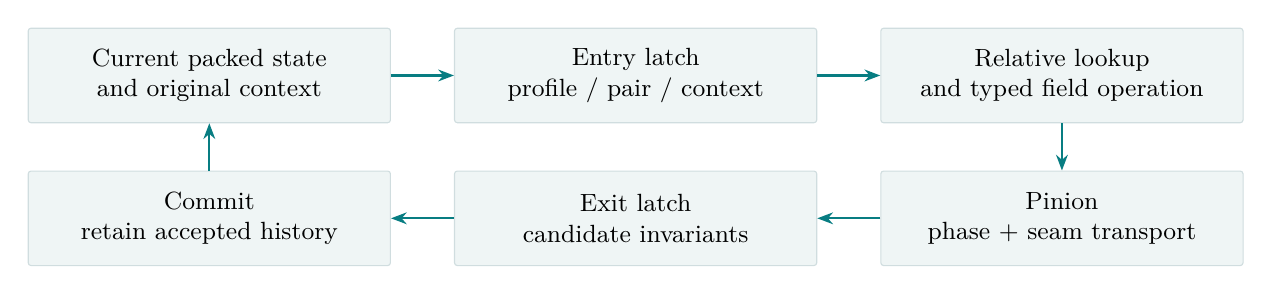
\begin{tikzpicture}[node distance=6mm and 8mm,box/.style={draw=rulecol,fill=wash,rounded corners=1pt,minimum width=46mm,minimum height=12mm,align=center,font=\small},arr/.style={-{Stealth[length=2mm]},teal,thick}]
\node[box] (state) {Current packed state\\and original context};
\node[box,right=of state] (entry) {Entry latch\\profile / pair / context};
\node[box,right=of entry] (lookup) {Relative lookup\\and typed field operation};
\node[box,below=of lookup] (pinion) {Pinion\\phase + seam transport};
\node[box,left=of pinion] (exit) {Exit latch\\candidate invariants};
\node[box,left=of exit] (commit) {Commit\\retain accepted history};
\draw[arr] (state)--(entry);\draw[arr] (entry)--(lookup);\draw[arr] (lookup)--(pinion);\draw[arr] (pinion)--(exit);\draw[arr] (exit)--(commit);\draw[arr] (commit)--(state);
\end{tikzpicture}
\end{center}
The diagram is a specification factorization. A valid implementation may fuse stages or use previously admitted immutable certificates, provided its observable classifications, results and failure behavior are unchanged. It need not recalculate an entire shortest-path field at every movement tick.

\subsection{The larger recurrence}
A grammar stage reads the prior bundle and original repaired state, emits a bounded transcript and primitives, constructs a \emph{candidate} bundle, then certifies it before admission. The output field cannot govern that same stage's earlier decisions. After GROW, the new bundle governs later operations. That is the source-bound relationship between self-reference and frozen evaluation. \krange{58}{64} \krange{88}{95} \kref{110}
\[
(\mathcal B_k,S_T,\text{original stage context})
\ \longrightarrow\ \text{finite derivation}\ \longrightarrow\ \widehat{\mathcal B}_{k+1}
\ \xrightarrow{\text{certify and admit}}\ \mathcal B_{k+1}.
\]

\begin{principle}
\textbf{The repeated unit is not a bare loop.} It is a typed operation together with the conditions under which its input, coupling and output are admitted. At the small scale it transports a packed state; at the larger scale it admits a generated field and continues the same owner.
\end{principle}

\sectionstart{Vocabulary that preserves the kernel}
\status{LP1 / TYPES BEFORE SYMBOLIC ASSOCIATION}
C links the hoop, pole, latch, pinion and packed SDF on pages 26--28. It later identifies the operators themselves with the represented field structure and insists that the LUT is self-referential. The following concordance preserves that line while using K to fix executable meanings. These are \emph{operational correspondences}, not claims that a glyph's appearance proves its mathematics. \crefrange{26}{28} \crefpage{212} \crefpage{226}

\begin{longtable}{L{28mm}L{53mm}L{72mm}}
\toprule
\textbf{Term}&\textbf{Meaning retained or introduced}&\textbf{Must remain distinct from}\\\midrule\endhead
Scalar $\phi$&Exact signed distance under a declared graph, zero set and side convention. \krange{12}{14}&One-bit side predicate; phase angle; physical strain without calibration.\\
Interval $\varphi$&Source interval/gating language. LG gives one optional finite phase-window binding.&K's scalar field, the golden ratio, or an unstated time scheduler.\\
Phase $R$ and $t$&Stored chart phase $R$; intrinsic phase $t=\sbit{\eta}R\bmod256$. \kref{44}&Logical time $T$, index derivation phase, or angular velocity.\\
Orientation $\eta$&One local reflection bit in live metadata. \krange{8}{20}&Parity bit, SDF sign, three-dimensional attitude or an independent actor.\\
Seam $\tau$&Relative reversing-edge action carried in an operator. \kref{20}&A scalar distance, time counter or spare live metadata bit.\\
Parity $p$&Even-popcount representation check for the complete 32-bit word. \kref{24}&Authentication, geometric certification or a lossless field code.\\
Pole / shaft / $\Psi$&Local traversal/eigen-axis or an emitted primitive's selected frame, under PX/DP/VP.&A mandatory external origin or a new physical mechanism.\\
Hinge / wire&Declared adjacency, frame transport or another explicitly typed relation. \kref{12}&The claim that every f8 tree link is a movement edge.\\
Latch&LP name for the profile's input/candidate/commit admissibility boundary.&A new opcode, unexplained intelligence, or spontaneous parity change.\\
Pinion&LP name for the exact phase-and-seam coupling, with a separate role for adapters.&An implicit call to arctangent or an uncalibrated force law.\\
J / KK&Source cut/join language; existing quotient identifications give one bounded stitching interpretation.&PX's matrix $J=\operatorname{diag}(1,-1)$; a universal CSG instruction.\\
f8&Versioned canonical lookup index with certified keys and row layout. \krange{40}{42}&Geometry, planner neighbor order or a proof of speed superiority.\\
T&Logical ordering in the kernel. Source side-view/operator usage is separately typed.&A fourth spatial component or a second intrinsic phase angle.\\
\bottomrule
\end{longtable}

\subsection{Same carrier, declared roles}
K's ``packet is the operator'' has a precise finite realization. In a live word, R is the current phase, G is the current node and B is its exact field value. In a STEP operator word, R is the phase increment, G is the destination and B is that destination's exact field value. Both use RP32, but their roles determine the interpretation. \krange{7}{8} \kref{15}

Instruction tapes are separately tagged: OG-TAPE32, TP-TAPE32 and VP-TAPE32 are not live RP32 state pairs. Their opcode width, continuation syntax and reserved bits follow their own contracts. W64 is another typed carrier, with a retained envelope. Preserving a common bit substrate does not permit decoding an instruction operand as a scalar field. \kref{58} \kref{73} \kref{87} \kref{111}

\subsection{Full mirror, not a second individual}
For metadata $a$ with seven payload bits,
\begin{align*}
v&=R+2^8G+2^{16}(B\bmod256)+2^{24}a,\\
\operatorname{pack}(R,G,B,a)&=v+2^{31}(\operatorname{popcount}(v)\bmod2),\\
M(\operatorname{pack}(R,G,B,a))&=\operatorname{pack}(-R\bmod256,G,B,a\oplus16),\\
\operatorname{Pair}(W)&=W+2^{32}M(W).
\end{align*}
The mirror preserves canonical $G$ and scalar $B$, reflects phase and toggles orientation. Every repack recomputes parity. The complete pair is the unit of state relation and active-payload eviction. \krange{8}{9}

\sectionstart{The latch--pinion kernel contract}
\status{LP2--LP7 / DERIVED FACTORIZATION OF EXISTING OBLIGATIONS}
\req{LP2}{Latch the admitted context before evaluation}
For an existing profile $\nu$, let $\mathcal D_\nu$ be the set of current-state/input pairs accepted for the selected operation after that profile's prescribed classification order. Its definition includes profile/version identity, retained dependencies, current epoch, legal metadata, pair/field consistency, operation eligibility and finite budgets where applicable. It does not merge all failures into a Boolean result.

The mathematical latch predicate is
\[
\Latch_\nu(S,e)=[(S,e)\in\mathcal D_\nu].
\]
Operationally, the profile retains the information that distinguishes INVALID, MISS, DEFER, WAIT, duplicate retry, ownership failure and other concrete outcomes. A declaration of this predicate is a specification of admissibility, not a claim that checking is free or that every check is implemented by one bit. \kref{5} \krange{72}{79}

\req{LP3}{Select from state, not from an unrelated action stream}
For standalone SDF v1/v2, retain
\begin{align*}
c(B)&=\begin{cases}0&B<0,\\1&B=0,\\2&B>0,\end{cases}\\
O_T&=L(G_T,c(B_T)),\\
L(i,c)&=\operatorname{pack}(\mathrm{turns}[i,c],\mathrm{routes}[i,c],
\phi(\mathrm{routes}[i,c]),\mathrm{STEP}\mid(\tau\ll6)).
\end{align*}
The seam term is absent in v1. In v2 it is derived from the authoritative seam set. FI/HP destinations instead come from their declared internal planner, and grammar F substeps from their declared field/phase rule. These mechanisms must not be conflated with the standalone table's fixed route columns. \kref{15} \kref{20} \kref{36} \kref{60}

A field-bound operator is therefore a typed word selected and checked in its proper world context. It does not need to contain its entire geometry, source code, calibration or certificate inside the 32-bit payload.

\req{LP4}{Use typed numerical lanes for field guidance}
Where HP applies, compute guidance from the certified departure field and the live intrinsic phase. Metadata, continuation flags and parity are not numerical vector components. The exact HP formulas, ranges, tie rules and search state remain binding. No repeated Hadamard transform is substituted for elementwise multiplication. \kref{11} \krange{44}{46}

\req{LP5}{Apply the pinion in the declared order}
The pinion's phase/orientation action is the existing K8 transport. With $\delta=O.R$, destination $j=O.G$ and relative seam bit $\tau$,
\begin{align}
\widetilde R&=(R+\sbit{\eta}\delta)\bmod256,\label{eq:depart}\\
R'&=\sbit{\tau}\widetilde R\bmod256,
&\eta'&=\eta\oplus\tau,\label{eq:seam}\\
W'&=\operatorname{pack}(R',j,\phi(j),\mathrm{STEP}\mid(\eta'\ll4)).\label{eq:repack}
\end{align}
K8 increments in the departure frame \emph{before} canonical seam reflection. Operator bit 6 does not leak into live metadata. The scalar field does not negate when orientation changes. These exact points are necessary to preserve the baseline fixtures. \kref{20}

Write the action as $\LP_{\delta,\tau}=S_\tau\circ U_\delta$, where
\[
U_\delta(R,\eta)=(R+\sbit{\eta}\delta,\eta),\qquad
S_\tau(R,\eta)=(\sbit{\tau}R,\eta\oplus\tau)
\]
with phase arithmetic modulo 256. The symbol $\LP$ is new notation for these existing equations; it is not the production component $P$ of $A_\nu$.

\req{LP6}{Latch the output against its own certificate and role}
Before accepting a candidate, require the selected profile's complete postconditions: legal destination, correct field value in the admitted world, exact metadata, valid parity, full mirror, expected energy/resource effects, and original-context identity. In a geometry change, the destination field and all index/operator resources must belong to the same certified candidate epoch.

Checking only the selected word's parity is insufficient. A well-formed word with a false $B$ must fail field admission; a correct final field with a false derivation must fail provenance admission. Which certificates can be cached and reused depends on immutable version identity. \kref{14} \krange{42}{47} \kref{113}

\req{LP7}{Commit only the complete admitted transition}
An accepted movement, planning event, GROW, index swap or W operation has its own atomicity and persistence boundary. A complete precommit rejection preserves the old semantic state; uncertainty after possible mutation closes the affected owner and invokes its recovery rules. A committed cleanup failure is not reported as a rejection. An unsaved W operation is not acknowledged as durably admitted. \kref{42} \kref{54} \kref{64} \kref{76}

\begin{principle}
\textbf{A latch is a contract boundary, not an arithmetic shortcut.} It may test structure, context, geometry, resource limits and commit state. Its meaning is the exact admission relation and failure behavior supplied by the selected profile.
\end{principle}

\sectionstart{Composition: following the pinion line exactly}
\status{NEW DEDUCTIONS FROM THE RETAINED PHASE AND SEAM EQUATIONS}
\subsection{The intrinsic quantity that survives a seam}
K defines intrinsic phase $t=\sbit{\eta}R\bmod256$. Applying equations \eqref{eq:depart}--\eqref{eq:seam} gives
\begin{align*}
t'&=\sbit{\eta\oplus\tau}R'\\
&=\sbit{\eta\oplus\tau}\sbit{\tau}(R+\sbit{\eta}\delta)\\
&=\sbit{\eta}R+\delta=t+\delta\pmod{256}.
\end{align*}
The seam changes the representation $(R,\eta)$, while the intrinsic increment remains $\delta$. The complete mirror also preserves $t$. These properties already underlie HP planning and its phase-bank selection. \kref{20} \krange{44}{45}

\begin{theorem}[Fixed-path pinion normal form]
Fix an already selected finite sequence of $n$ legal transitions, with increments $\delta_0,\ldots,\delta_{n-1}$ and seam bits $\tau_0,\ldots,\tau_{n-1}$. Its phase/orientation result is
\[
\boxed{
 t_n=t_0+\sum_{i=0}^{n-1}\delta_i\pmod{256},\quad
 \eta_n=\eta_0\oplus\bigoplus_{i=0}^{n-1}\tau_i,\quad
 R_n=\sbit{\eta_n}t_n\pmod{256}.}
\]
\end{theorem}
\begin{proof}
One step satisfies the intrinsic increment identity above and toggles orientation by its seam bit. Induction accumulates the increments and XORs the seam bits. The defining relation $t_n=\sbit{\eta_n}R_n$ then recovers $R_n$. Repacking with the separately established destination, field and metadata recovers the complete pair.
\end{proof}

\textbf{What this proves.} Multiple local chart reversals can be accounted for without inventing a different global phase operator. The recurring pinions have one exact compositional numerical meaning under K8.

\textbf{What this does not prove.} The increment sequence is itself state/field dependent; HP costs depend on intermediate phase; latches may reject intermediate operations; new observations can change planning; a grammar stage may emit geometry at intermediate positions. Summing increments is not permission to skip those dependencies or to compress an entire semantic history into $(t_n,\eta_n)$.

\subsection{The mirror is coherent through a pinion}
\begin{theorem}[Full-mirror transport coherence]
Under the scalar-field convention and the same selected operator, both views of a valid pair yield full mirrors after K8 transport.
\end{theorem}
\begin{proof}
Let $s=\sbit{\eta}$. Starting from the mirrored phase/orientation gives departure value $-R-s\delta$ and post-seam phase $-\sbit{\tau}(R+s\delta)$. This is the negative of the left result. The right orientation is $(\eta\oplus\tau)\oplus1$. Both results retain the same destination and scalar field, and deterministic parity repacking completes the mirror relation.
\end{proof}
This restates the K1 mirror theorem in the pinion vocabulary. For a general operation that does not commute with $M$, K's conjugate right action $M\circ U\circ M^{-1}$ remains the required construction. \kref{9} \kref{20}

\subsection{Guarded composition, not unrestricted multiplication}
For two partial admitted transitions $F_1,F_2$, the composite exists exactly when
\[
(S,e_1)\in\mathcal D_1
\quad\text{and}\quad
(F_1(S,e_1),e_2)\in\mathcal D_2,
\]
where $F_1(S,e_1)$ denotes its accepted successor state. A failed first result is propagated according to the profile; it is not an input state for the second operation. A macro-operation that must be atomic prepares and checks its complete candidate before committing; it does not retroactively hide an earlier independently admitted event.

\begin{principle}
\textbf{One correct meaning, several legitimate descriptions.} Word arithmetic, a field interpreter, a tree-backed lookup and a graphical description can agree when they preserve the same admitted transitions and outputs. Agreement is established by a refinement relation, not by reusing the same symbols or obtaining a similar picture.
\end{principle}

\sectionstart{The latch, the hoop and the JKK zipper}
\status{SOURCE CONCORDANCE / EXPLICIT INTERPRETIVE LIMITS}
\subsection{What the author's prompts actually fix}
C's sequence is specific: an open radial degree in the hoop/pole construction; the latch/pinion/SDF connection; J as a half-set cut and KK as a zipper; and a valve that prevents an operator from passing in the wrong context. Those prompts motivate an interface, its correspondence and its admission condition. They do not supply a complete new bit layout or a numerical phase interval. \crefrange{26}{29}

K binds the operative pieces separately: graph adjacency and field support; finite quotient identifications; seam action; full-pair validity; and tagged rejection with preserved state. This revision connects the vocabulary to those definitions. It does not adopt the archived AI response's claim that a wrong time necessarily creates a one-bit fault or that closing a software gate physically stops time. \kref{12} \krange{19}{24}

\subsection{A decorated edge is a precise local coupling}
For explanation, write a field operator's local support as
\[
\mathfrak e=(\nu,k,i,j,\delta,\tau,\mathsf{role},\mathcal D,\mathcal Q),
\]
where $i,j$ are canonical geometric identities, $\mathcal D$ its input domain and $\mathcal Q$ its output obligation. This is a mathematical descriptor assembled from existing context and rules. It is not an assertion that RP32 stores all nine items.

The \emph{hinge} is the permitted relation $i\to j$; the \emph{pinion} is its exact phase/frame action; the \emph{latch} is admissibility of the correspondence and result. The same descriptor pattern can describe an elementary movement or, with another explicit role, a bounded candidate-world admission.

\subsection{Cut and zipper: an existing quotient interpretation}
For the Klein profile, the matching boundary representatives are already fixed by
\[
(u,v+H)\sim(u,v),\qquad (u+W,v)\sim(u,-v).
\]
Reading an exposed chart boundary as a ``cut'' and the declared representative matching as a ``zipper'' is a bounded interpretation of C's JKK language. K supplies the decisive extra structure: cells, edge/face incidences, cyclic vertex links, orientation cover and the transported packed state. A list of reversing graph edges alone is not a certified Klein surface. \krange{19}{20}

No arbitrary cut/glue algorithm is introduced here. A future JKK graph-rewrite profile would still need exact ports, multiplicity, matching maps, topology checks, field reconstruction, budgets and commit semantics. Until then, JKK is a source-level name for these specified roles, not an executable universal CSG command.

\subsection{The ``third piece'' belongs at the correct interface}
C later asks whether Cartesian-to-polar conversion is the pinion. K does not use that conversion as OTAN2; it already defines OTAN2 as a relative finite phase action. A sensor or legacy-coordinate adapter may convert external measurements into admitted phase or scale codes, but its units, quantization, calibration and original inputs must be declared. That adapter is an additional coupling role, not a replacement for K8. \crefpage{259} \kref{6} \kref{25}

\begin{scopebox}
\textbf{Notation policy.} This edition writes source J as $J_{\mathrm{cut}}$ when discussing cutting, and $J_{\mathrm{frame}}$ for the reflection matrix used by PX. KK denotes the source's joining role. No equality between these objects is implied by their shared letter or visual form.
\end{scopebox}

\sectionstart{Optional finite phase-window latch}
\status{LG1--LG8 / NEW FORMAL PRIMITIVE / NOT AN EXISTING RUNTIME POLICY}
The source interval language can be made exact without altering scalar $\phi$ or silently adding a gate to a verified policy. The following is one proposed numerical binding. The corpus does not uniquely force these endpoints or this cyclic-window convention. Existing FI, HP, GD, OG, DP, VP and W contracts remain as retained unless a separately versioned future policy explicitly adopts it.

\req{LG1}{A total, finite guard primitive}
Define the standalone function
\[
\mathsf{Window}(a,\ell,t)=
\begin{cases}
1 & ((t-a)\bmod256)<\ell,\\
0 & \text{otherwise},
\end{cases}
\qquad a,t\in\{0,\ldots,255\},\ \ell\in\{0,\ldots,256\}.
\]
All arguments are strict integers. $\ell=0$ admits no phases; $\ell=256$ admits all phases. Otherwise the interval includes its start and excludes the endpoint after $\ell$ steps. This uses a finite cyclic order, not real-time elapsed duration or physical clock jitter.

\req{LG2}{Evaluate intrinsic phase, not an arbitrary chart phase}
At a prospective departure, use $t=\sbit{\eta}R\bmod256$ from the validated live pair. A gate using raw $R$ would generally disagree across mirrored views. Index $\mathsf{phase\_origin}$ is not a live phase input.

\req{LG3}{Retain the full gate identity}
A future adopting policy must retain $(a,\ell)$ or the immutable rule that derives them from admitted input. The guard's type/version, phase source and evaluation point are semantic choices. They cannot be hidden in spare RP32 bits, an undocumented W selector, or an unrecorded wall clock.

\req{LG4}{Place the gate before the guarded evaluation}
Under the proposed departure-window convention, validate the input pair, resolve the selected operation and gate parameters from the same admitted context, then evaluate the guard. Only the successful branch evaluates the guarded candidate operation. Recompute and validate output parity as usual; parity itself is not the window parameter.

\req{LG5}{Do not invent a failure policy}
The primitive returns a Boolean only. An adopting transition profile must separately choose a tagged result for a closed window, its priority relative to other failures, and whether any explicit waiting event can advance a clock. Existing W's error alphabet and retry ordering are not extended by this mathematical definition.

\req{LG6}{Freeze the interpretation for a candidate stage}
A gate used inside grammar interpretation must read the prior certified world and the current hypothetical cursor in that stage, or another explicitly named source. It cannot use a partially generated field. A gate on owner admission must be distinguished from a gate on a hypothetical F substep.

\req{LG7}{Preserve full-open compatibility}
For the standalone guard, $\mathsf{Window}(a,256,t)=1$ for every valid $a,t$. A future extension that only adds this guard must prove reduction to the unchanged predecessor semantics when the window is full. That proof must include classifications and histories, not merely final phase.

\req{LG8}{Require a new integration contract before deployment}
No existing manifest key, opcode, transport field or API has been modified. Production adoption requires an explicit version, schema, blocked-window result, policy priority, resource bound, host/device parity and replay tests. The independent checks in this edition establish the finite guard's arithmetic, not that integration.

\begin{theorem}[Window cardinality and mirror invariance]
Every valid window admits exactly $\ell$ of the 256 intrinsic phases. Applying a full RP32 mirror leaves its Boolean result unchanged.
\end{theorem}
\begin{proof}
Translation $t\mapsto(t-a)\bmod256$ is a permutation of the 256 residues. Exactly $\ell$ lie below $\ell$. Full mirroring sends $(R,\eta)$ to $(-R,\eta\oplus1)$, preserving $\sbit{\eta}R$ modulo 256; therefore it preserves the guard input and result.
\end{proof}

\textbf{Literal wrap example.} $(a,\ell)=(252,8)$ admits $252,253,254,255,0,1,2,3$. A state at intrinsic phase 254 passes; phase 4 fails. This example specifies a proposed interval convention, not the intended parameters of an unspecified physical latch.

\sectionstart{Exact fields and typed Hadamard guidance}
\status{RETAINED NUMERICS / EXPLICIT FIELD-FAMILY DISTINCTIONS}
\subsection{Distance is certified independently of representation}
The finite field contract uses a connected undirected graph, positive edge weights, a nonempty boundary and declared sides $\sigma\in\{-1,0,+1\}$. Its field is
\[
D(v)=\min_{z\in Z}d(v,z),\qquad \phi(v)=\sigma(v)D(v).
\]
No edge directly connects opposite nonzero signs. The exact SDF range is $[-127,127]$; $-128$ is unused and overflow rejects rather than saturates. The scalar field pulls back unchanged to both local-frame sheets. \krange{13}{14} \kref{21}

The independent distance certificate requires correct signs/zeros/ranges plus
\[
|D(u)-D(v)|\le w(u,v),\qquad
D(v)=w(v,u)+D(u)\text{ for some neighbor }u\text{ when }v\notin Z.
\]
The witness strictly decreases distance until reaching $Z$; telescoping yields an attaining path. The edge inequalities lower-bound every other boundary-reaching path. Thus the result is exact for the declared graph and boundary. This geometric check is separate from parity and mirror validity. \kref{14}

\subsection{Three constructions that must not be collapsed}
\begin{tabularx}{\textwidth}{L{24mm}Y}
\toprule
\textbf{Profile}&\textbf{Authoritative geometry-to-field meaning}\\\midrule
OG4&$q(v)=\min_i(d_K(v,c_i)-r_i)$; $\sigma=\operatorname{sign}q$; $Z=\{q=0\}$; redistance to $Z$. The primitive list retains order and duplicates. \kref{61}\\
DP5&OR-union $U$ of closed intrinsic balls and projected taper footprints; $Z=\{v\in U:\exists j\sim v,\ j\notin U\}$; zero on $Z$, negative on $U\setminus Z$, positive outside; redistance. \kref{90}\\
VP5&Same inner occupied boundary convention, but $U$ comes from projected sampled three-dimensional spheres, cones and pyramids on $K\times S^1$. Six-neighbor graph distances define the field. \kref{106}\\\bottomrule
\end{tabularx}

\textbf{Compatibility consequence.} Even an S-only DP tape can differ from an old OG tape, because the boundary convention changed under an explicit new profile. ``Union first, then redistance'' does not authorize replacing OG4's zero set with DP5's inner boundary. Nor does it authorize using a minimum of old signed fields as the new exact field. \kref{86} \kref{90}

This is a material refinement of the earlier corpus-only reconstruction: its broad account of union/boundary extraction is now resolved into the distinct OG, DP and VP contracts rather than treated as one interchangeable procedure.

\subsection{The existing product already has an exact three-factor form}
HP2 defines, in the canonical departure frame,
\begin{align*}
g&=(\phi(u^+)-\phi(u^-),\ \phi(v^+)-\phi(v^-)),\\
A&=gg^{\mathsf T},\qquad
\Psi=\frac{g}{\gcd(|g_u|,|g_v|)}\quad(g\ne0),\\
t&=\sbit{\eta}R\bmod256,\qquad b_{\mathrm{bank}}=\lfloor t/64\rfloor,\\
q_i&=\mathsf{gain}[b_{\mathrm{bank}},i](1+\Psi_i^2)g_i.
\end{align*}
For $g=0$, PX fixes $\Psi=(1,0)$ and $q=0$. This can be written without changing its meaning as
\[
\boxed{q=\mathsf{gain}[b_{\mathrm{bank}}]\odot(\mathbf1+\Psi\odot\Psi)\odot g.}
\]
This factorization uses successive \emph{elementwise} products. It is a direct algebraic restatement of HP2, not a new Hadamard-transform or quantum interpretation of ``double.'' Products use widened signed integer arithmetic with scale $f=0$ and no clipping. \kref{39} \kref{44}

\subsection{Guidance changes the next action}
For a cardinal geometric edge $e$,
\[
\mathsf{penalty}=\max_i|q_i|-q\cdot e,\qquad
\mathsf{cost}=1+|\phi(\mathrm{dest})|+\mathsf{hazard}(\mathrm{dest})+\mathsf{penalty}.
\]
The component bound is $|q_i|\le40$, penalty is $0..80$ and total edge cost is $1..335$. Intrinsic phase selects the bank \emph{before} the departure increment. The planner must retain $(G,t,\mathrm{hops})$, because equal nodes reached with different phases can have different futures. \krange{44}{45}

VP8 extends the same typed idea to three components, eight banks and six cardinal neighbors under its new profile. It does not add a second phase angle, reuse the old five-component key ABI, or claim a measured volume runtime. \krange{102}{109}

\sectionstart{Grammar, f8 and the frozen-stage rule}
\status{LP8--LP9 / SELF-REFERENCE WITH EXPLICIT DEPENDENCIES}
\req{LP8}{Keep within-stage evaluation acyclic in the new field}
A stage begins from the original repaired EMIT pair and prior certified field. Changing the hypothetical cursor's opcode to STEP does not create a second owner. Parallel rewriting reads only the previous finite word; a first matching rule wins; newly emitted symbols wait until the next generation. Ordered tape interpretation then reads the fixed prior field throughout. \krange{58}{60}

The dependency order is
\begin{align*}
\text{original context}&\to\text{rewritten tape}\to\text{cursor/branch transcript}\\
&\to\text{primitive descriptors}\to\text{candidate field}\\
&\to\text{candidate resources}.
\end{align*}
K's self-reference is the fact that updated state participates in the \emph{next} lookup and interpretation. It is not circular authority for a candidate to certify itself with an undefined future field. This provides a precise kernel reading alongside C's insistence on both packed self-reference and frozen structure. \kref{6} \kref{60} \kref{88} \crefpage{192} \crefpage{226}

\subsection{Complete branch restoration}
PUSH saves the complete cursor pair, radius, scale and enclosing branch path. POP restores exactly those items, including phase, scalar field and orientation after a seam crossing. Program position, work counters, previously emitted primitives, transcript order, energy and owner history do not rewind. Saving only $\eta$ is not a complete frame. \kref{60} \kref{88} \kref{110}

The final hypothetical cursor does not automatically become the live owner. OG/DP/VP preserve owner $G,R,\eta$, replace $B$ with the newly certified field at $G$, debit the declared cost and select a new target. GD instead maps $G$ through its explicit dyadic embedding. Those operations have different numerical and identity contracts. \kref{51} \kref{62} \kref{93} \kref{114}

\req{LP9}{Never substitute a storage relation for a geometric relation}
PX orders canonical descriptors by
\[
(\Psi_u+2,\Psi_v+2,\rho,\theta,G),\qquad
\rho=\lfloor\log_2(d_{\mathrm{anchor}}+1)\rfloor.
\]
The lower median of each sorted interval becomes a tree node, emitted in preorder. Tree rows are storage addresses; $G$ remains the canonical geometric node ID. Actual lookup must walk the tree and verify the returned identity, but tree links are not motion edges. \krange{40}{41}

An index rebuild changes a certified storage bundle, not the field, route cost, lexical tie, search cursor, energy or history. A geometry GROW changes semantic context and invalidates the prescribed observations/search/cache. The two kinds of replacement must never share an ambiguous ``update'' operation. \kref{42} \kref{47} \kref{54}

\subsection{What ``precedence'' means in the realized kernel}
C asks for procedural grammar and packed operator precedence. K realizes deterministic order through explicit token arities, first-match production priority, previous-generation reads, tape order, complete stack behavior, field-before-resource construction and admission-before-commit. The four-entry precedence list supplied by the archived AI is not substituted for those actual grammar rules. \crefpage{58} \krange{58}{64}

\begin{scopebox}
\textbf{Coordinate-free does not mean address-free.} K permits canonical node names, array indices, temporary charts and integer texture rows. Their role is representational. A purported translation that removes these objects without replacing their identity, ordering and lookup obligations has not preserved the kernel. \kref{4} \kref{12}
\end{scopebox}

\sectionstart{Time, retained state and durable latching}
\status{LP10--LP11 / THE SAME INDIVIDUAL CONTINUES}
\req{LP10}{Retain every output-affecting original dependency}
Exact regeneration is evaluation of the same versioned expression with the same original arguments. Eviction removes a derived active copy, not the last copy of arbitrary external information. Baselines, rules, observations, stage contexts and required prefixes have separate retention policies. A missing non-derived input produces the profile's missing-dependency result; it is not synthesized from a later clock. \kref{18} \kref{37}

\[
\mathsf{Regen}(d)=\mathsf{Eval}_\nu(\omega,\mathsf{rules},T_{\mathrm{original}},
\mathsf{path},\mathsf{original\ inputs}).
\]
For complete 64-bit pairs, the preallocated active payload is $8C$ bytes. Total memory additionally includes geometry, scalar fields, indexes, operator atlases, recipes, observations, journals, planning and runtime overhead. Cache capacity can affect residency without changing decisions; a budget that changes admitted time or semantics must remain part of the original context. \kref{18} \kref{47} \kref{59}

\subsection{The clocks do not substitute for each other}
\begin{tabularx}{\textwidth}{L{36mm}Y}
\toprule
\textbf{Quantity}&\textbf{Meaning and update rule}\\\midrule
Intrinsic phase $t$&Cyclic $0..255$ state quantity advanced by departure increments. Not a logical counter.\\
Agent cycle / $T$&Logical agent progression; accepted planning DEFER can affect the original GROW time.\\
Geometry epoch $k$&Admitted generated-world identity. Old observations are interpreted in their original geometry.\\
Index epoch&Certified storage version. A storage-only reindex does not become a movement or grammar event.\\
Producer epoch/sequence&Input namespace and delivery ordering. Not a chart orientation or clock carry.\\
W clock&$T_W=\mathsf{clock\_origin}+n$ over a bounded 48-bit range; every new admitted W operation advances $n$.\\
Device ticks&Executor-local action counter, reset on GROW under the declared implementation. Not W time or agent cycle.\\\bottomrule
\end{tabularx}
\krange{55}{59} \kref{70} \kref{77}

\subsection{Stage prefixes and historical-sample prefixes differ}
OG/DP/VP stage context hashes the events \emph{before} the admitting GROW, avoiding a circular digest through that event's receipt. A historical generated-world sample qualifies its original admission prefix \emph{through} GROW. Both use the same retained canonical JSON convention but different boundaries. The digest binds context; it does not supply authentication or a spatial seed. \kref{55} \kref{63} \kref{113}

\req{LP11}{Preserve the forward interface and its private recovery}
W admits exactly IGNITE, ADVANCE, RESIZE, INVALIDATE and EMIT. A new operation advances W time; only ADVANCE invokes an agent step. A latest exact retry is classified before dynamic checks that may have changed after success, returns no historical payload and does not dispatch a second emission or action. Static schema/source checks still precede retry classification. \krange{70}{79}

INVALIDATE is an explicit validated removal of selected active pairs, preserving unaffected order and retained dependencies. A rejected backward request does not automatically change parity or invalidate memory. Private R recovery reconstructs the complete W operation/cache sequence and original agent history without exposing a public historical-read operation. \krange{71}{76}

\begin{principle}
\textbf{The durable latch closes at acknowledgment.} W does not acknowledge an operation until its archive is saved under the ownership contract. A save or device outcome that may be uncertain closes the owner. A fresh session resolves the durable prefix rather than guessing that the old state remained active. \kref{76}
\end{principle}

\sectionstart{Equivalence, preservation and proof obligations}
\status{LP12 / WHAT MAKES ANOTHER FORMALIZATION CORRECT}
\req{LP12}{Preserve meaning through an explicit refinement}
Retain K's implementation relation, extended here only to make the observation boundary explicit:
\[
\operatorname{Decode}_\alpha\!\bigl(\operatorname{Exec}_\alpha(
\operatorname{Encode}_\alpha(S),e)\bigr)=F_\nu(S,e).
\]
The equality includes selected result classification, canonical output, admitted state and the profile's retained-history obligations. A word round trip alone does not establish it. An implementation may fuse arithmetic, change storage order or use another exact field algorithm only when these observables agree. \kref{16} \kref{23}

\subsection{State preservation under the LP factorization}
Let $\Inv_\nu$ be the selected profile's invariant: role-correct words, exact $G/B$ relation, permitted topology and destinations, legal phase/metadata, complete mirrors, consistent context and remaining finite budgets.

\begin{theorem}[Conditional preservation through latched pinions]
Suppose $\Inv_\nu(S_0)$, each entry latch enforces its stated premises, selected operations use the admitted bundle, each successful candidate satisfies the exit obligation, and commit installs precisely that candidate with the prescribed history. Then every accepted successor satisfies $\Inv_\nu$.
\end{theorem}
\begin{proof}
For one accepted step, the input premises license its operator. Its exact arithmetic and transported destination produce the checked candidate. The exit obligation establishes the invariant of that candidate; faithful commit installs it. Induction over accepted transitions establishes the assertion. Rejected candidates do not enter the induction; uncertain execution follows the profile's failure/recovery contract rather than being counted as a successful transition.
\end{proof}
This is an organized application of K's G3, K1 and I3 arguments, not a new unconditional infallibility claim. The substantive premises remain obligations of the producer, certifier and runtime. \kref{15} \kref{20} \kref{22}

\subsection{Representation invariance needs the complete policy}
K's graph-isomorphism statement transports weights, sides, boundary and operator rules. To extend that statement to planning or grammar, also transport the semantic orders, tie-breaking rules and input identities on which they depend. Merely renaming nodes and then imposing a different lexical order can change a tied decision; that is not the same transported policy. \kref{12} \kref{36} \kref{45}

Bit-identical replay is stronger than equivalent decoded geometry. It retains the original canonical manifest and output convention. Conversely, a legal full mirror can represent the same intrinsic phase but be a different \emph{owned ordered pair}; W validates the actual owner, not any mirror-swapped replacement. \kref{12} \kref{73}

\subsection{Storage refinement versus semantic change}
\begin{tabularx}{\textwidth}{L{48mm}Y}
\toprule
\textbf{Candidate change}&\textbf{Required classification}\\\midrule
Different certified f8 rows or index sign/origin&Storage refinement only if every semantic decision, event, field and pending search is preserved.\\
Different active FIFO capacity&Residency change if derivations and decisions remain equal. W may still record different capacity/cache witnesses.\\
Different HP gains or added nontrivial phase gate&New semantic policy or admitted control; it cannot inherit the old policy's complete history claim.\\
Different search quantum&Retained semantic input where DEFER changes original grammar time; identical whole missions are not promised.\\
Different boundary convention&New field/profile identity, as already demonstrated by OG versus DP.\\
Different external calibration&New admitted adapter context; neither bit determinism nor a field certificate proves unchanged physical meaning.\\\bottomrule
\end{tabularx}
\kref{42} \kref{59} \kref{86} \kref{99}

\subsection{The remaining proof boundary}
A finite transition proof, an arithmetic reference, implementation testing, fault-model assurance and physical validation are different claims. The conditional infallibility contract remains: a completely specified bounded profile, valid initial state, ordered inputs and faithful execution yield a defined result and preserved invariants. Self-reference does not waive any of these premises. \krange{22}{25}

\sectionstart{Worked trace and discriminating witnesses}
\status{SOURCE VECTORS / INDEPENDENTLY RECOMPUTED SUBSET}
\subsection{One reversing seam, in full detail}
The HP reference uses the 4 by 5 Klein recipe, phase 250, initial energy 100 and repair cost 5. Its source-field turns are $[11,53,137]$. After the first move the owner is at $G=4$, $R=5$, $B=-1$, $\eta=0$. The next admitted movement is $4\to16$ across a reversing seam. \kref{48}
\[
\delta=11,\quad\tau=1,\quad\widetilde R=5+11=16,\quad
R'=-16\bmod256=240,\quad\eta'=1.
\]
Intrinsic phase is $t'=(-1)240\bmod256=16$. The new scalar field is $B'=\phi(16)=0$, not a sign-flipped old value. The exact pair is \code{81001010910010F0}. Its left word carries $R=240$ and orientation 1; the right word is the complete mirror. This is the pinion arithmetic and exit invariant in one literal transition.

\begin{tabularx}{\textwidth}{L{27mm}L{34mm}Y L{17mm}}
\toprule
\textbf{Action}&\textbf{Known route / cost}&\textbf{Actual pair}&\textbf{Energy}\\\midrule
MOVE 1&$[4,3,17]$ / 7&\code{11FF04FB01FF0405}&98\\
Seam MOVE&$[16,17]$ / 7&\code{81001010910010F0}&93\\
MOVE 3&$[17]$ / 2&\code{81011145910111BB}&91\\
REPAIR&Repair cost 5&\code{06011145160111BB}&86\\\bottomrule
\end{tabularx}
The fresh hazard 70 at node 3 from cycle 2 explains the replanned route in K. The independent revision check recomputes the displayed path costs and packed actions; it does not claim to rerun the original observation endpoint or its complete mission fixture. \kref{48}

\subsection{Counterexamples that rule out superficially similar replacements}
\begin{longtable}{L{35mm}L{73mm}L{45mm}}
\toprule
\textbf{Proposed substitution}&\textbf{Literal discriminator}&\textbf{Consequence}\\\midrule\endhead
Drop phase from search&At start 0, target 10, phase 128, hop bound 12: $(G,t,h)$ yields $[1,6,5,10]$, cost 10; $(G,h)$ yields $[5,10]$, cost 11. \kref{48}&Phase is part of the planning state, not display metadata.\\
Shift old distance during growth&3 by 5, centre 1, radius 3: old $B(0)=-3$. Doubled geometry gives $B'(0)=-4$, not $-6$. \kref{51}&Generate and redistance the new boundary.\\
Use OG union margin as distance&3 by 3, balls $(0,2),(4,2)$: margin and exact field differ at nodes 2 and 3. \kref{65}&Equal signs do not imply equal boundary distance.\\
Treat every DP field as old OG&A taper on 8 by 8 has zero vertex 38 with no negative neighbor. Every positive-radius OG zero-margin vertex has a negative neighbor. \kref{90}&The field families have distinct semantics.\\
Treat cone and pyramid as the same solid&VP witness at $(s,t,r)=(2,1,1)$ lies in the slope-1/2 pyramid, not the cone. \kref{104}&Equal axial sections do not identify full volumes.\\
Use wrapped u32 squares&A height-2 cone, slope 65535/65534, charges 75 sites but has 40 wrong membership decisions under native-u32 wrapping. \kref{112}&Small work bounds do not eliminate wide-arithmetic obligations.\\
Use parity as geometry proof&A valid-parity, fully mirrored replacement can still carry a false $B$ for its node. \krange{14}{24}&Representation and geometric admission remain separate.\\\bottomrule
\end{longtable}

\Needspace{12\baselineskip}\subsection{The same carrier still distinguishes three solids}
For K's 6 by 6 by 6 witness, the independently recomputed vertex/cube counts are:
\begin{center}
\begin{tabular}{lrrrr}
\toprule
&Occupied&Boundary&Interior&Complete cubes\\\midrule
Cone&29&27&2&4\\
Pyramid&45&43&2&8\\
Sphere&33&26&7&8\\\bottomrule
\end{tabular}
\end{center}
These are mathematical expectations of VP3/VP5, not evidence that VP's GPU, one-owner mission or Wv3 runtime has been implemented. \kref{104} \kref{117}

\sectionstart{Evidence ledger and revision checks}
\status{HISTORICAL IMPLEMENTATION / NEW LOCAL ARITHMETIC / FORMAL SCOPE}
\subsection{Retained implementation chronology}
The following counts are reported in the supplied kernel. Each row refers to its own retained capture, not to a sum of all previous rows or a new execution during this revision.

\begin{tabularx}{\textwidth}{L{24mm}r r Y}
\toprule
\textbf{Capture}&\textbf{Tests}&\textbf{GPU methods}&\textbf{Source and scope}\\\midrule
SDF&262&21&Retained earlier field capture. \kref{27}\\
Klein&311&28&Finite quotient/cover and seam profile. \kref{27}\\
FI&368&41&Integrated field agent. \kref{38}\\
PX&421&55&Local Psi and f8; 20 PX checks. \kref{43}\\
HP&479&77&Phase-directed routing; 15 checks. \kref{49}\\
GD&546&107&Dyadic growth; 16 checks. \kref{57}\\
OG&623&136&Parameterized organogram; 15 checks. \krange{67}{68}\\
W&698&145&Forward interface and private recovery; 14 checks. \krange{82}{83}\\
DP / Wv2&796&179&Directional sections; 15 DP and 8 Wv2 checks. \krange{98}{100}\\
VP / Wv3&\multicolumn{2}{l}{\emph{No admitted runtime capture}}&Formal contract and independent expected values; runtime remains required. \krange{101}{117}\\\bottomrule
\end{tabularx}

K's recorded hardware/software descriptions and benchmark scopes are retained in the appendix. This revision has not independently retrieved the repository source inventories, report files or hardware. The cited identifiers and hashes are therefore \emph{reported evidence provenance}, not fresh attestations of an inspected checkout. The actual uploaded PDF bytes have been hashed separately for this document. \kref{27} \kref{30} \kref{100}

\subsection{Nineteen newly executed reference groups}
The independent program uses only the Python standard library. Its scope is deliberately narrower than the original implementation: direct formulas, finite enumerations, graph searches, literal field constructions and byte codecs. It has no device execution, disk-session ownership, network endpoint or fault-injected persistence adapter.

\begin{longtable}{L{10mm}L{77mm}r L{35mm}}
\toprule
\textbf{ID}&\textbf{Passed reference group}&\textbf{Cases}&\textbf{Basis}\\\midrule\endhead
V01&RP32 lane sweeps / mirror&896&K 7--8\\
V02&Three literal packed pairs&3&K 8\\
V03&Single-bit detection / typed zero&259&K 24\\
V04&Exhaustive K8 phase and mirror&262,144&K 6, 8, 20\\
V05&Fixed-path two-pinion normal form&49,152&New deduction\\
V06&Weighted v1 field / 64-tick trace&65&K 27, 31\\
V07&Klein v2 / 64-tick seam trace&64&K 21\\
V08&Local Psi / degeneracy / frames&100&K 39\\
V09&PX key and lower-median orders&20&K 40--43\\
V10&HP reference costs / owned pairs&4&K 48\\
V11&Phase-retaining search witness&2&K 48\\
V12&OG redistance / forged field&10&K 14, 61, 65\\
V13&DP taper / OG distinction&64&K 90\\
V14&GD changed-boundary distance&2&K 51\\
V15&VP three-solid occupancy&3&K 104; formal\\
V16&VP limbs / u32 overflow witness&65,617&K 112; formal\\
V17&W byte order / fragment lengths&6&K 73, 80\\
V18&LG window cardinality / wrapping&65,792&New; optional\\
V19&LG window mirror invariance&131,072&New; optional\\
\bottomrule
\end{longtable}


The exhaustive phase group covers every $256\times2\times256\times2=262{,}144$ combination of stored phase, orientation, increment and seam bit. The optional-window cardinality group covers all 65,792 start/length pairs and evaluates all 16,842,752 phase memberships; its separate mirror group covers 131,072 cases. Other groups are selected exhaustive subdomains or literal vectors, not exhaustive coverage of every RP32 word or every possible program history.

\subsection{What the checks add}
They expose transcription or composition errors in this edition, independently reproduce selected K literals, and test the new path/window arithmetic. They do not upgrade VP from formal-only, establish that LG has a runtime policy, or transfer the original 796-test/GPU status to newly written code. Proofs in this document remain human-readable mathematical arguments, not a proof-assistant certificate.

\begin{scopebox}
\textbf{Reproduction.} Extract \code{independent_reference.py} and run:
\begin{lstlisting}
python independent_reference.py --output independent_checks.json
\end{lstlisting}
The original repository commands remain on the retained K pages. They were not executed in this revision. The source script, generated JSON and exact source-PDF hashes are included as attachments and in the companion bundle.
\end{scopebox}

\sectionstart{Acceptance, maturity and extension register}
\status{NO IMPLIED COMPLETION / EXPLICIT NEXT CONTRACTS}
\subsection{Acceptance of the document upgrade}
A reader can check this edition against the following concrete obligations. The entire baseline is present; existing numerical constants and profile identities are not silently changed; C quotations are attributed to author prompts or AI responses as appropriate; the LP synthesis cites K's definitions; the LG guard is marked new and optional; all new reported local checks have retained code/results; and linked K references resolve to the original numbered pages.

\begin{tabularx}{\textwidth}{L{37mm}Y}
\toprule
\textbf{Layer}&\textbf{Status in Revision 16}\\\midrule
Core RP32 / SDF / Klein / PX / HP&Exact definitions retained. Historical bounded CPU/GPU implementation evidence reported by K. Selected arithmetic/vector checks additionally reproduced here.\\
FI/GD/OG/DP and W/Wv2&Full contracts and recorded captures retained. New explanatory linkage does not replace their runtime requirements or claim a fresh end-to-end rerun.\\
LP latch/pinion synthesis&New derived integration vocabulary, compositional proofs and conformance organization; existing profile semantics unchanged.\\
LG phase-window primitive&New finite mathematical function and conditional integration requirements. Local arithmetic checked; production policy and device integration not supplied.\\
VP and Wv3&Formal-only source contract retained. Selected occupancy and wide-arithmetic expectations reproduced; full runtime acceptance still required.\\
Physical adapters and broader claims&Unbound or separately specified applications. No new claim of physical sensing, universal immunity, computational universality or comparative hardware advantage.\\\bottomrule
\end{tabularx}

\subsection{Unresolved source terms stay explicit}
\textbf{Arbitrary JKK cuts and joins.} No general executable topology-rewrite syntax is supplied by the selected corpus passages. Port identities, matching maps, orientation action, cells, budgets and candidate certification must be bound before adoption.

\textbf{The intended $\varphi$ window.} LG is one proposal, not a recovered unique interval from C. A physical or logical-time gate could be different and would need its own retained parameters and interaction policy.

\textbf{Mechanical pinions or a Cartesian input adapter.} K8 is numerical frame transport. A real gear, transducer or conversion from measured coordinates needs a separate adapter/model. This document does not derive mechanical forces from parity.

\textbf{Global Psi, arbitrary graph growth and universality.} Local rank-one $gg^{\mathsf T}$ and finite generative profiles retain their actual scope. A new spectral operator, production family or universality theorem requires its own definitions and evidence. \kref{39} \kref{102} \kref{117}

\subsection{An adoption path that does not damage verified behavior}
First adopt the documentation-only LP terminology and retain all original schemas. Then select any genuinely new semantics, such as LG, under a new policy/version with an exact failure rule. Prepare an independent full reference before implementation. Finally run both that new profile's conformance and the untouched earlier regression fixtures, capturing source, device, outputs and failure behavior separately. This follows K's formal-first progression; it does not presume the new feature already works in the old runtime.

\sectionstart{Corpus-to-kernel concordance}
\status{AUTHOR PROMPTS / REALIZED MEANINGS / REMAINING CHOICES}
The quotations below are short excerpts from the user's labelled prompts in C. They are used as design intent. The exact realization is supplied by K or, where explicitly indicated, proposed in this revision.

\begin{longtable}{L{25mm}L{67mm}L{61mm}}
\toprule
\textbf{Corpus locator}&\textbf{Author's stated line}&\textbf{Kernel destination / upgrade treatment}\\\midrule\endhead
p.6, prompt 6&``lower case phi interval places the parity bit around the hadamard products''&Keep phase/orientation and representation checks typed. K pp.6,20,24,44 supply actual arithmetic; LG adds only a proposed interval guard.\\
p.26, prompt 5&``a pole that latches to a rim''; ``an open radial degree''&LP names interface, coupling and admission roles. No literal hoop geometry or unique angle is inferred.\\
p.27, prompt 6&``latch pole pinion double hadamard packed eigenvector axis signed distance fields''&K pp.12,15,20,39,44 distinguish support, transport, local axis and product. LP exposes their dependency order.\\
p.28, prompt 7&``J means half set cut and KK is the zipper''&Existing quotient matching and frame transport provide a bounded interpretation; arbitrary JKK graph surgery remains unbound.\\
p.28, prompt 8; p.29, prompt 9&JKK as a valve; then ``logic ? how can JKK have logic?''&LP uses explicit admissibility relations and tagged results, not an anthropomorphic decision-maker or automatic physical corruption.\\
p.58, prompt 7&``formal grammar (procedural grammar) L-system along the binary search tree''&K pp.58--64 define productions/tape/stack; K pp.40--42 define a separate storage tree. Preserve both relations.\\
p.192, prompt 16&``never dynamically always statically frozen''&K pp.60,88,110 fix the prior field during a stage. C's phrase alone is not a prohibition on every later admitted GROW.\\
p.212, prompt 3&``the semantic operators are themselves signed distance fields''&K pp.7,12,15 give shared carrier, geometric support and field-selected executable words; no universal untyped identity is imposed.\\
p.213, prompt 5&``taking away the coordinates (spaces) leaving only signed distance field''&K pp.4,12 distinguish intrinsic semantics from temporary charts and memory addresses.\\
p.220, prompt 7&``every operator is a same structure packed operators''&K pp.7--8,58,73,87,111 require carrier/profile/role decoding. Shared representation does not collapse tape and state types.\\
p.222, prompt 9&``middle outs via the binary search tree via double packed pinion''&K pp.40--43 bind lower-median f8 and exact keys; phase/seam action remains K8, not a tree-edge move.\\
p.226, prompt 13&``my entire architecture is based around the log encoded polar LUT that is self referential and packed''&K p.6 gives $q_T\to O_T\to X_{T+1}\to q_{T+1}$; LP preserves that closed dependency sequence.\\
p.259, prompt 28&``conversion from cartesian to polar coordinates is the pinion? the missing third piece?''&Separate an external adapter role from intrinsic OTAN2/K8. No arctangent replacement is introduced.\\
p.271, prompt 14&``1bit words as letters procedural grammars''&K pp.24,58--59 retain Boolean predicates, exact scalar magnitude, typed instructions and finite rewriting as distinct levels.\\\bottomrule
\end{longtable}

\subsection{Archived AI translations not inherited as kernel definitions}
C's page-27 quantum-Hadamard account, page-28 smooth-union formula, page-202 double-pass transform, page-226 zero-cost global synchronization claims and later physical material analogies are not used as executable premises. K already fixes the applicable operator, geometry, resource and adapter contracts. This is source-priority discipline, not a replacement of the author's kernel with outside theory. \krange{11}{25}

In particular, the double-pass matrix displayed on C p.202 satisfies $H^2=I$ in exact arithmetic. That archived transform cannot be the nontrivial elementwise HP operator. The identity follows by multiplying the displayed $2\times2$ matrix; the retained HP formula is the authority for this edition. \crefpage{202} \kref{44}

\sectionstart{Source identity and reproducibility}
\status{EXACT UPLOADED FILES / EMBEDDED SUPPORTING ARTIFACTS}
\subsection{Supplied primary documents}
\textbf{K.} Tom Klootwijk, \emph{Ontological Deterministic Computing: The Infallible Contract}, TK-LPLUT-2.0 Revision 15, 26 September 2026. Uploaded filename: \nolinkurl{Tom_Klootwijk_Ontological_Deterministic_Computing_v2.0.pdf}. 117 pages; 460,376 bytes.
\begin{lstlisting}
SHA-256
68951a1c6c63e1e9e454045fc0c9d043d
3b2e6afb3c6ec9235ec284341cd9253
\end{lstlisting}
\textbf{C.} \emph{BookNook / Google AI Mode: Conversations \& doodles}, 29 September 2026. Uploaded filename: \nolinkurl{BookNook-Google-AI-Mode-2026-09-29-Tom Klootwijk en Jitske K-K(1).pdf}. 278 pages; 16,159,441 bytes. C records 42 captured conversations and separately labelled prompts/responses. \crefpage{1}
\begin{lstlisting}
SHA-256
3f339bbda7627487742368734995a1028
818a166291217e881d1be175871dd15
\end{lstlisting}
Join each two-line digest with no spaces. These are hashes of the actual supplied PDFs, not the earlier source-PDF hashes reported inside K, nor a signature of authorship.

\clearpage\subsection{What the PDF retains}
All 117 K pages follow this upgrade with their original text and layout. The original K file is also embedded as an attachment, preserving its bytes independently of page import. The source corpus is not duplicated wholesale; its relevant author prompts are traced through the concordance and its supplied-file hash. Earlier source PDFs and repository files named inside K were not independently available as attached bytes and are not claimed to be bundled.

\begin{tabularx}{\textwidth}{L{63mm}Y}
\toprule
\textbf{Embedded attachment}&\textbf{Purpose}\\\midrule
\code{revision15-original.pdf}&Byte-preserved authoritative source K.\\
\code{independent_reference.py}&Standalone CPU arithmetic/check program written for this revision.\\
\code{independent_checks.json}&Actual 19-group results, case scopes, runtime environment and script hash.\\
\code{source_manifest.json}&Supplied filenames, byte lengths, page counts and SHA-256 digests.\\
\code{README.txt}&Reproduction instructions and exact scope limitations.\\\bottomrule
\end{tabularx}

\subsection{Original software and references}
The retained baseline gives module paths, conformance commands, source/report identities and technical references on K pp.26--34, 49, 57, 67--68, 82--83 and 98--100. These remain references to the original development artifacts. No outside research or current API specification has been substituted into this source-grounded document upgrade.

\begin{principle}
\textbf{The resulting line.} Certified relations determine the field; the field and live phase determine an operation; exact pinion transport proposes the next representation; latches admit the result and its history. Grammar repeats the construction at a larger scale while retaining the prior context. That is the integrated kernel reading preserved throughout this edition.
\end{principle}

\clearpage
\phantomsection\section*{Retained authoritative baseline}
\addcontentsline{toc}{section}{Retained authoritative baseline: Revision 15 (117 pages)}
\status{K-1 THROUGH K-117 / ORIGINAL PAGE BODIES UNCHANGED}
The following pages reproduce the complete uploaded Revision 15 kernel. They are part of this upgraded reading edition, not excerpts. Original requirements, proof statements, literal vectors, schemas, evidence counts and historical status labels remain intact.

\begin{tabularx}{\textwidth}{L{30mm}Y}
\toprule
\textbf{K pages}&\textbf{Retained section family}\\\midrule
1--34&Charter, exact core, SDF/Klein, conditional infallibility, implementation map, history and source provenance.\\
35--38&FI1--FI8: field-guided individual, observations, planning, action and replay.\\
39--43&PX1--PX8: local Psi, canonical f8 keys, actual lookup and atomic storage replacement.\\
44--49&HP1--HP8: phase-directed Hadamard costs, planning, atlas and recorded implementation.\\
50--57&GD1--GD8: finite dyadic geometry growth, original-prefix identity and measured continuation.\\
58--68&OG1--OG8: parameterized grammar, branch restoration, union-margin field and measured device generation.\\
69--83&W1--W8: forward operations, clock, typed carrier, latest retry, private recovery and recorded evidence.\\
84--97&DP1--DP10: original formal-first directional-section contract.\\
98--100&Later DP/Wv2 implementation capture: 796 tests and its separate historical scope.\\
101--117&VP1--VP16: three-dimensional volume, new ABI, wide arithmetic and formal-only acceptance contract.\\\bottomrule
\end{tabularx}

\vspace{8mm}
\textbf{Read chronology, not isolated labels.} The DP appendix's preimplementation labels are retained because they are historical page bodies. The later DP evidence does not rewrite those earlier statements, and it does not establish that the still later VP runtime exists. The new evidence ledger resolves this progression without altering the source.
\vfill
{\small\color{muted}End of Revision 16 integration pages. The original baseline begins on the next page.}
\clearpage
\renewcommand{\thepage}{K-\arabic{page}}
\setcounter{page}{1}
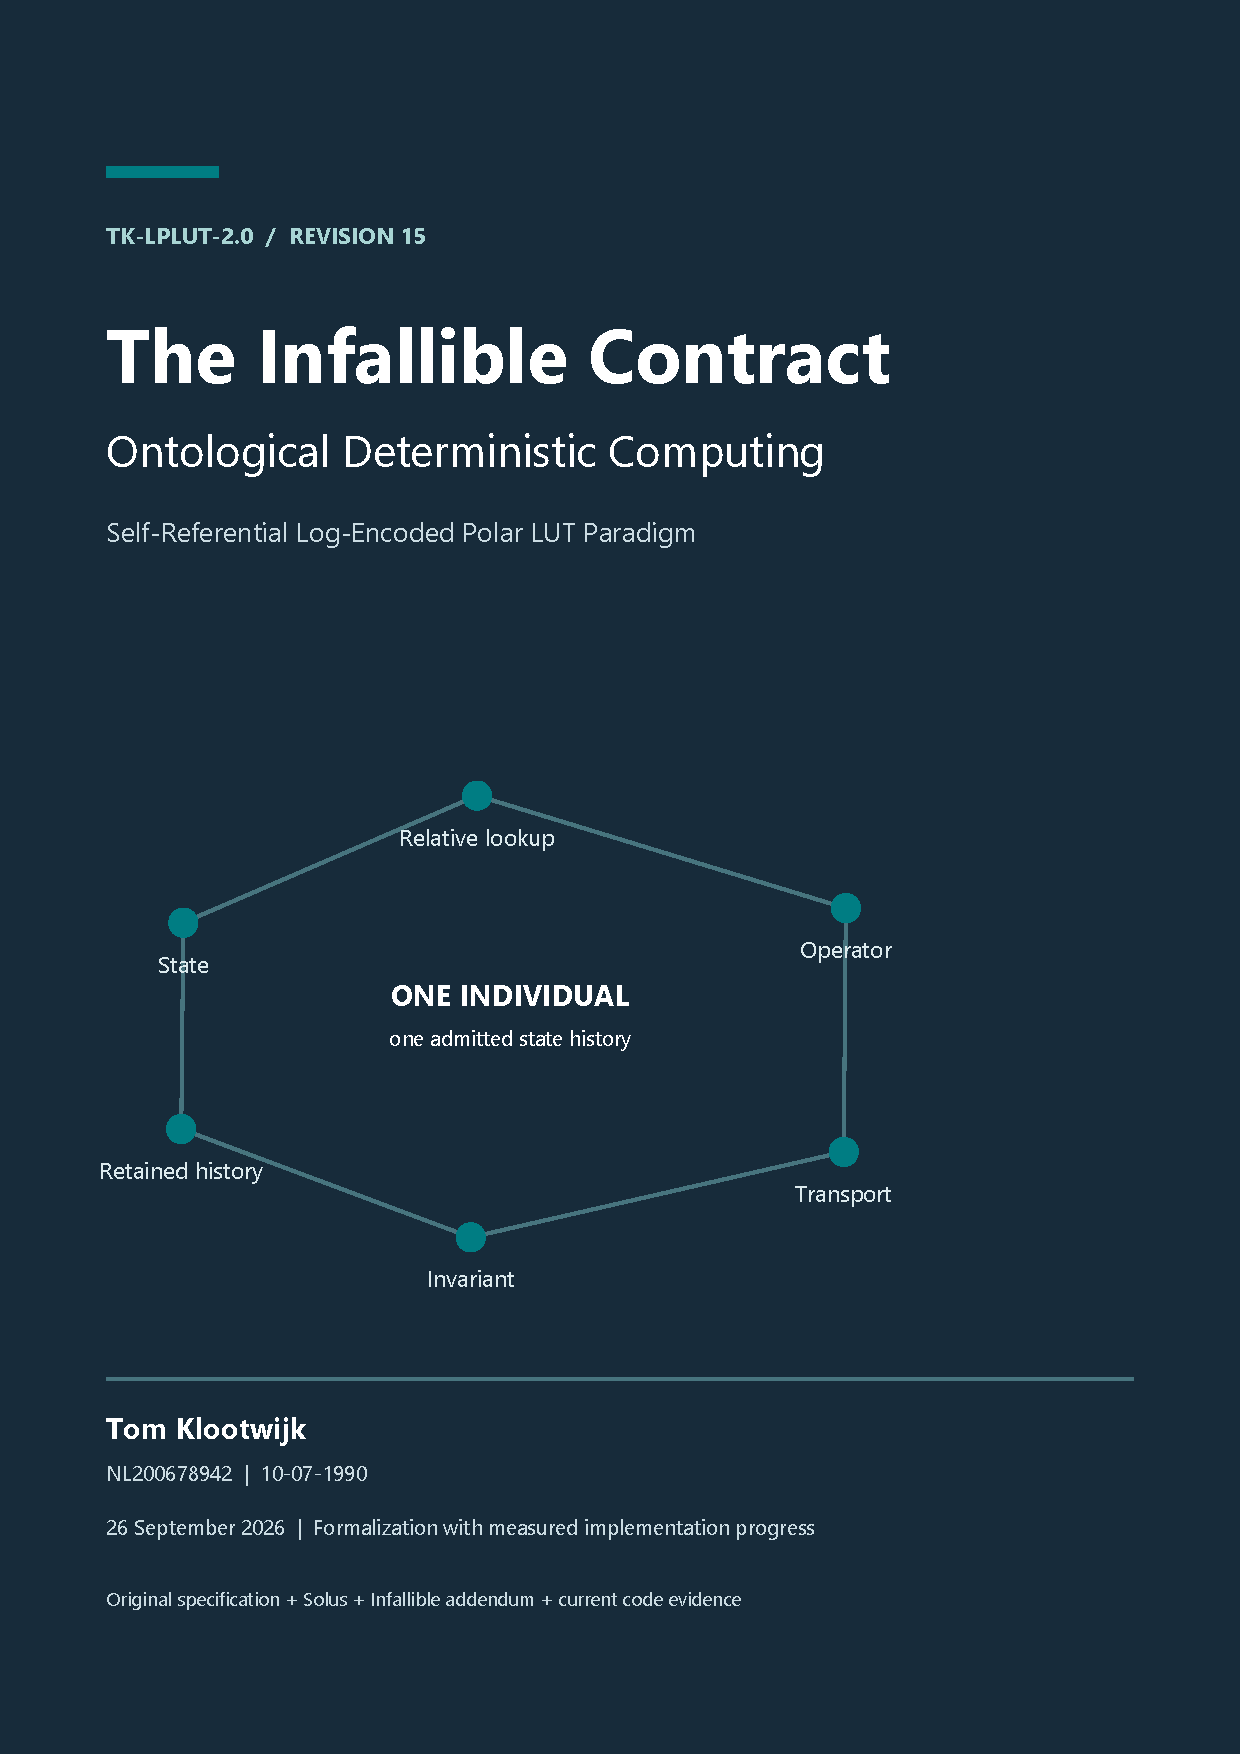
\includepdf[pages=-,pagecommand={\thispagestyle{empty}},link=true,linkname=baseline,addtotoc={1,section,1,Revision 15 - complete authoritative source,orig-source,4,subsection,2,Charter and exact core,orig-core,13,subsection,2,Exact SDF and certificate,orig-sdf,19,subsection,2,Klein quotient and transport,orig-klein,35,subsection,2,FI - Field-guided individual,orig-fi,39,subsection,2,PX - Psi and f8,orig-px,44,subsection,2,HP - Hadamard routing,orig-hp,50,subsection,2,GD - Dyadic growth,orig-gd,58,subsection,2,OG - Parameterized organogram,orig-og,69,subsection,2,W - Forward interface,orig-w,84,subsection,2,DP - Directional contract,orig-dp,98,subsection,2,DP and Wv2 implementation evidence,orig-dpevidence,101,subsection,2,VP - Formal-only volume contract,orig-vp}]{kernel_original.pdf}
\end{document}
